\section{Introduction}
\label{sec:intro}

% %!TEX root = ../../main.tex
\begin{figure*}[!t]
    \centering 
    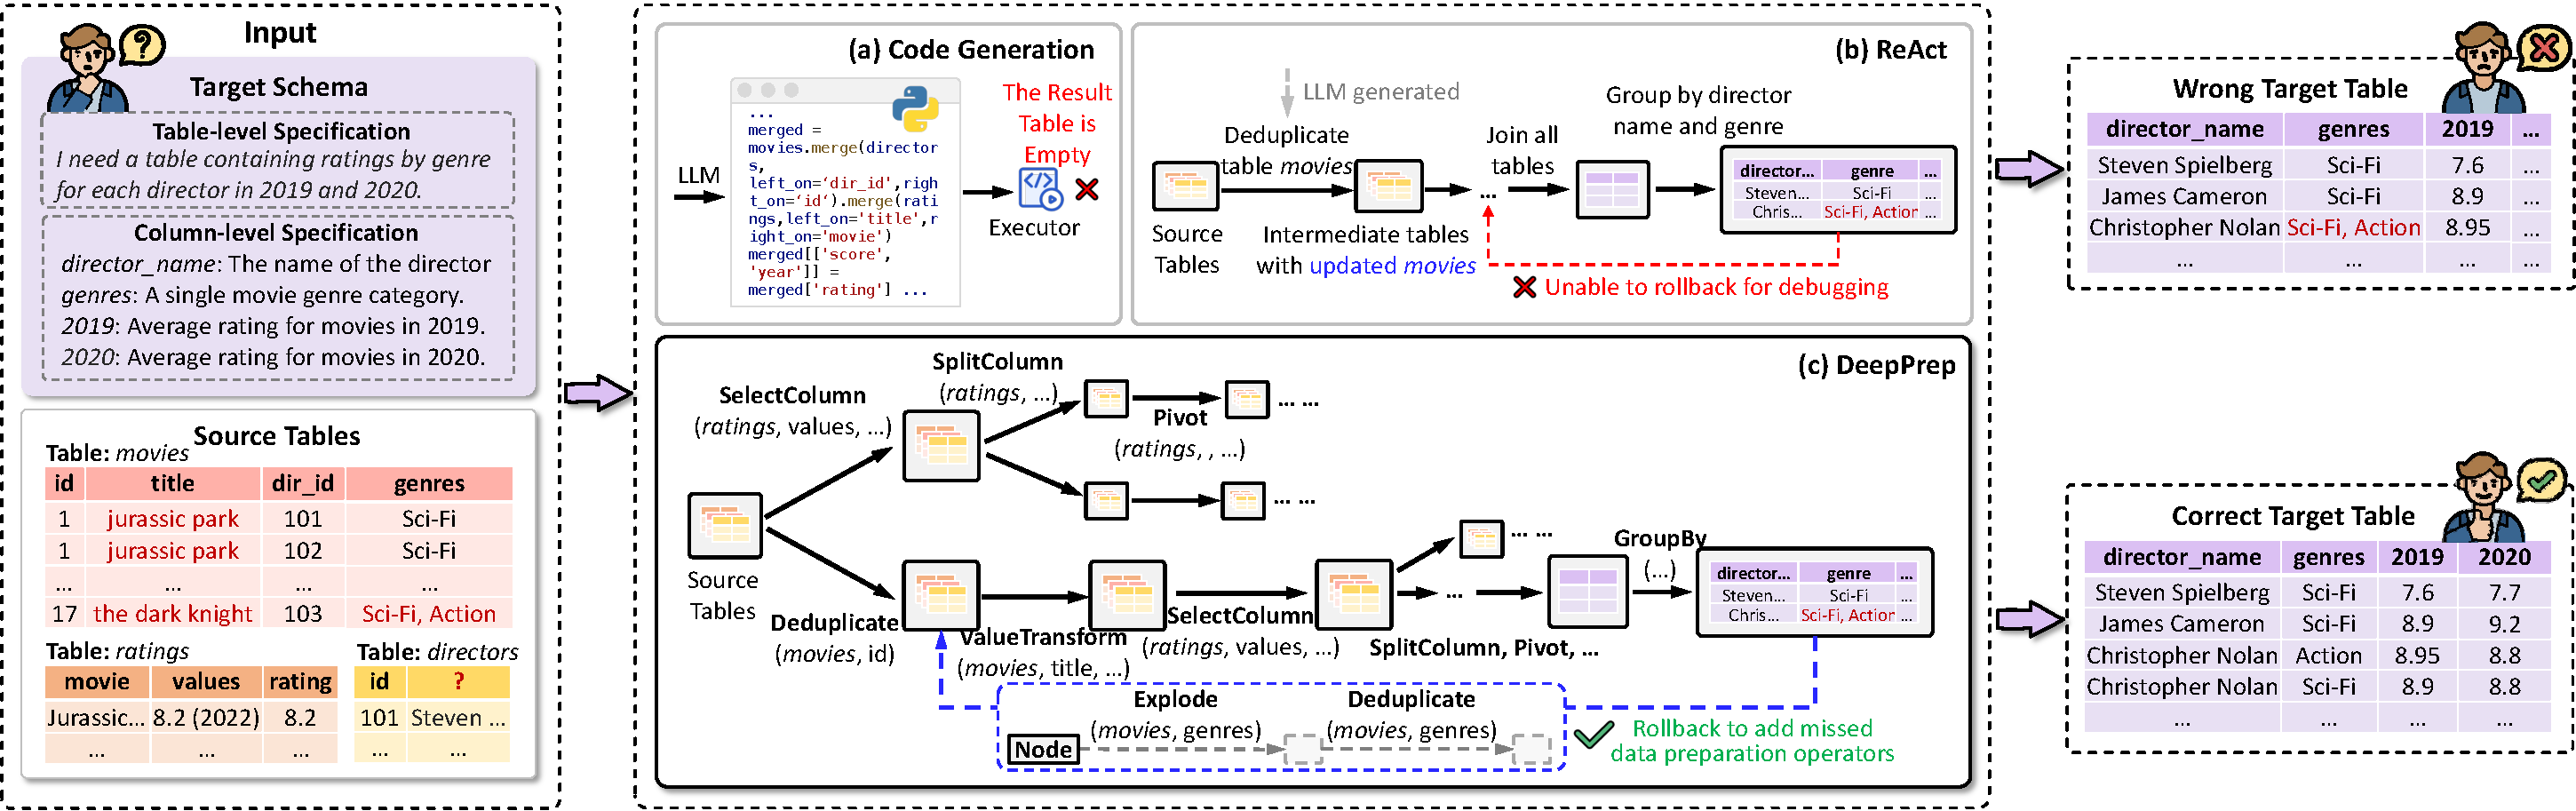
\includegraphics[width=0.95\textwidth]{figures/fig/introduction_example.pdf}
    \vspace{-1em}
    \caption{An illustrative example highlighting the core idea of \sys.
(a) Code generation makes decisions without grounding in intermediate execution results.
(b) ReAct-style approaches follow linear reasoning with limited ability to revise earlier decisions.
(c) \sys applies a tree-based structured exploration, which enables backtracking to resolve non-local errors.
    }
    \label{fig:introduction_example}
    \vspace{-1em}
\end{figure*}

% \fmh{(High Level) Task: Table to table transformation with NL supervision. Make the reader convince that this the the naive and necessary process under the application scenerio.}
Data preparation (DP), including column transformation, table transformation and data cleaning, underpins modern Business Intelligence (BI), Extract-Transform-Load (ETL), and analytics workflows. Typical enterprise pipelines require composing multi-step transformations over heterogeneous tabular sources to normalize schemas, fix errors, reconcile entities, and produce analysis-ready tables.

% \fmh{Current Approaches Limitation. Fail to orchestrate the DP operations. Previous work only focus on subtask. Thus, it is naive to use LLM-based React Prompting framework.}
\stitle{Current Approaches and Their Limitations.} The state-of-the-art (SOTA) results in DP are achieved through task-specific deep learning methodologies and rule-based systems. These methods involve specialized models trained on extensive datasets for narrow sub-problems such as string normalization~\cite{DBLP:journals/pvldb/LiYLFT25}, entity deduplication~\cite{DBLP:conf/icde/FanHFC00024}, or table reconstruction~\cite{yang2021auto}. However, current approaches to DP suffer from two fundamental limitations that significantly constrain their practical applicability.

\etitle{(1) Narrow Task-Specific Design.} Previous DP methods are narrowly scoped, targeting isolated sub-problems rather than end-to-end workflows. For instance, methods like~\cite{DBLP:journals/pvldb/LiYLFT25, DBLP:conf/icde/FanHFC00024} focus solely on data cleaning tasks, while ~\cite{yang2021auto} addresses only table transformation. it causes two fundamental issues: (1) incompatible tool composition where specialized methods use different input/output formats and conflicting assumptions, preventing seamless integration, and (2) lack of global optimization where locally optimal decisions in individual components lead to globally suboptimal pipelines. 

% \fmh{Method to improve orchestration ability: Tree Exploration (Debug), Data Construction (Long chain data)}
% \fmh{Data Construction renames: highlight ``Long Chain''}

\etitle{(2) Ground Truth Dependency.} Current DP methods rely on supervised learning paradigms that require ground truth target tables to train models for generating correct transformation sequences. These approaches assume access to paired input-output table examples where the desired final state is explicitly provided during training~\cite{DBLP:conf/sigmod/YanH20}. However, in real-world scenarios, practitioners typically have only source tables and high-level target table description expressed in natural language, without knowing the exact structure or content of the target output tables. This dependency on unavailable supervision signals severely limits the practical deployment of existing DP solutions.

\stitle{Unified End-to-End Data Preparation with Natural Language Specification.} Meanwhile, large language models (LLMs) have demonstrated remarkable capabilities in understanding NL instructions and generating executable code under various tasks. This presents an opportunity to address the aforementioned limitations through NL-guided End-to-End data preparation. 

\stitle{Technical challenges.} Despite this promising potential, applying LLMs to end-to-end DP presents unique technical challenges that differ from conventional code generation tasks.

{(C1) Lack of End-to-End Training Data with NL Specification.} Existing datasets only cover narrow DP sub-tasks without large-scale natural language to multi-step DP workflow mappings. For example, xxx

{(C2) Long-Chain Reasoning Challenge.} DP workflows require complex multi-step reasoning with error recovery capabilities that exceed current LLM inference paradigms. In unified End-to-End DP with NL specification, systems must navigate vast search spaces to find correct operation combinations. Consider a typical scenario with 15 fundamental DP operations where a task requires 10-step operations, which yields $15^{10} \approx 5.8 \times 10^{11}$ possible combinations. The search space expands exponentially when considering operation parameters. Current LLMs struggle with such vast sequential decision-making, often getting trapped in suboptimal paths without effective backtracking mechanisms~\cite{xxx}.

\stitle{\sys: An Agentic Model for Unified and User-Friendly Data Preparation.} In this paper, we propose \sys, which features two key ideas to address the above two challenges. 

To address (C1), we propose a verifiable and scalable data construction methodology. Specifically, we define a unified operator space covering comprehensive DP operations including column transformation, table reconstruction, and data cleaning. Starting with clean tables from existing NL2SQL datasets that reflect real-world data analysis scenarios, we systematically apply inverse operators (e.g., introducing typos, duplicates, schema inconsistencies) to generate "dirty" variants, while using LLMs to generate corresponding natural language target descriptions based on the clean table schemas. This reverse-engineering approach ensures both verifiability and scalability, providing large-scale, diverse training data that resolves the scarcity of NL-to-DP workflow mappings.

% \fmh{ReAct will miss some operators and be trapped in one wrong operator.}
To address (C2), we propose a Trainable Tree-based Exploration Framework for effecient and accurate DP operation generation.
Unlike traditional ReAct-style sequential reasoning, our framework generates multiple candidate operator sequences simultaneously at each exploration step rather than single operations, avoiding local optima inherent in greedy approaches. The framework supports on-the-fly execution of candidate sequences with immediate feedback, enabling backtracking to previous states and exploration of alternative paths when encountering errors or suboptimal results. This multi-path parallel exploration combined with execution feedback efficiently navigates the exponential search space of operator combinations. To further enhance long-horizon reasoning capabilities, we complement this with a post-training scheme that combines supervised fine-tuning on verifiable trajectories with reinforcement learning using carefully designed partial rewards.

\stitle{Contributions.} Our contributions are summarized as follows.

% \vspace{1mm} \noindent
(1) We introduce a verifiable data construction methodology that defines a unified operator space and generates large-scale NL-to-DP workflow training data through inverse transformations, addressing the scarcity of end-to-end DP supervision (Section~\ref{sec:xxx}).

% \vspace{0.5mm} \noindent
(2) We propose \sys, a trainable tree-based exploration framework that enables multi-path parallel search with execution feedback and backtracking, combined with a post-training scheme using SFT and partial reward RL for enhanced long-horizon reasoning (Section~\ref{sec:xxx}). 

% \vspace{0.5mm} \noindent
(3) We conduct comprehensive evaluation demonstrating that \sys achieves state-of-the-art performance on both our constructed corpus and public DP benchmarks, improving end-to-end success rates by xxx while reducing search cost by xxx compared to existing approaches (Section~\ref{sec:xxx}).


% \begin{table}[t]
  \centering
  \caption{\bf Statistics of datasets.}
  \vspace{-1em}
  \label{tbl:datasets}
  \resizebox{0.93\columnwidth}{!}{
    % 修改列定义：添加了第5列 'c'
    \begin{tabular}{|c||c|c|c|c|}
      \hline
      % 修改表头：添加了 "# Op types" 列，同样使用 multirow 跨两行
      \multirow{2}{*}{\textbf{Dataset}} & \multicolumn{2}{c|}{\textbf{Statistics}} & \multirow{2}{*}{\textbf{Pipeline Length}} & \multirow{2}{*}{\textbf{\# Op Types}} \\ \cline{2-3}
       & \textbf{\# Train} & \textbf{\# Test} & & \\
      \hline \hline
      
      \textbf{Synth-Spider} 
      & 6,788 & 2,008 & 1$\sim$28 & 31 \\ \hline
      
      \textbf{Synth-Bird} 
      & - & 1,150 & 2$\sim$25 & 31 \\ \hline
      
      \textbf{Parrot} ~\cite{ge2025text}
      & 13,965 & 1,365 & 1$\sim$8 & 17 \\
      \hline

      \revise{\textbf{Buildings}~\cite{sharma2023automatic}}
      & \revise{-} & \revise{105} & \revise{-} & \revise{-} \\
      \hline
    \end{tabular}
  }
  \vspace{-1em}
\end{table}

